\documentclass{article}

\usepackage{graphicx}
\usepackage{float}

\title{Note on "RetLLM-E: Retrieval-Prompt Strategy for Question-Answering on Student Discussion Forums"}
\author{Chancharik Mitra, Mihran Miroyan, Rishi Jain, Vedant Kumud,\\ Gireeja Ranade, Narges Norouzi}
\date{\today}

\begin{document}

\maketitle

\section{Which problem is addressed by the paper?}

This paper focuses on using Large Language Models(LLMs) to support teaching assistants in answering questions on specific aspects, like course-assignments QA. 
Not only give thorough answers, but guide students to the right direction, by providing prompts to help them think critically and solve the problem themselves.

\section{Why is it important?}

\begin{itemize}
    \item LLMs are weak in answering specific questions about a course's content or assignments.
    \item In educational settings, the relevance and factuality are of utmost importance. In contrast, hallucination often occurs in LLMs.
\end{itemize}

\section{How is it solved?}

\begin{itemize}
    \item Each student question is passed to both Q\&A retrieval and document retrieval modules.
    \item The Q\&A retrieval module uses \textbf{multi-qa-mpnet-basedot-v1} as a backbone. This paper use the nearest neighbor approach to identify the top three Q\&A pairs closest to the original student question from the bank of processed Q\&A pairs.
    \item This paper uses a document retrieval pipeline with an \textbf{InstructorXL} backbone.
    \item leverage prompt engineering to incorporate both the Q\&A and document context into a prompt template designed to enhance the pedagogical value of the generated response.
    \item prompt the LLaMA-2-13B-chat model with weighted sampling from the top five token.
\end{itemize}


\begin{figure}[H]
    \centering
    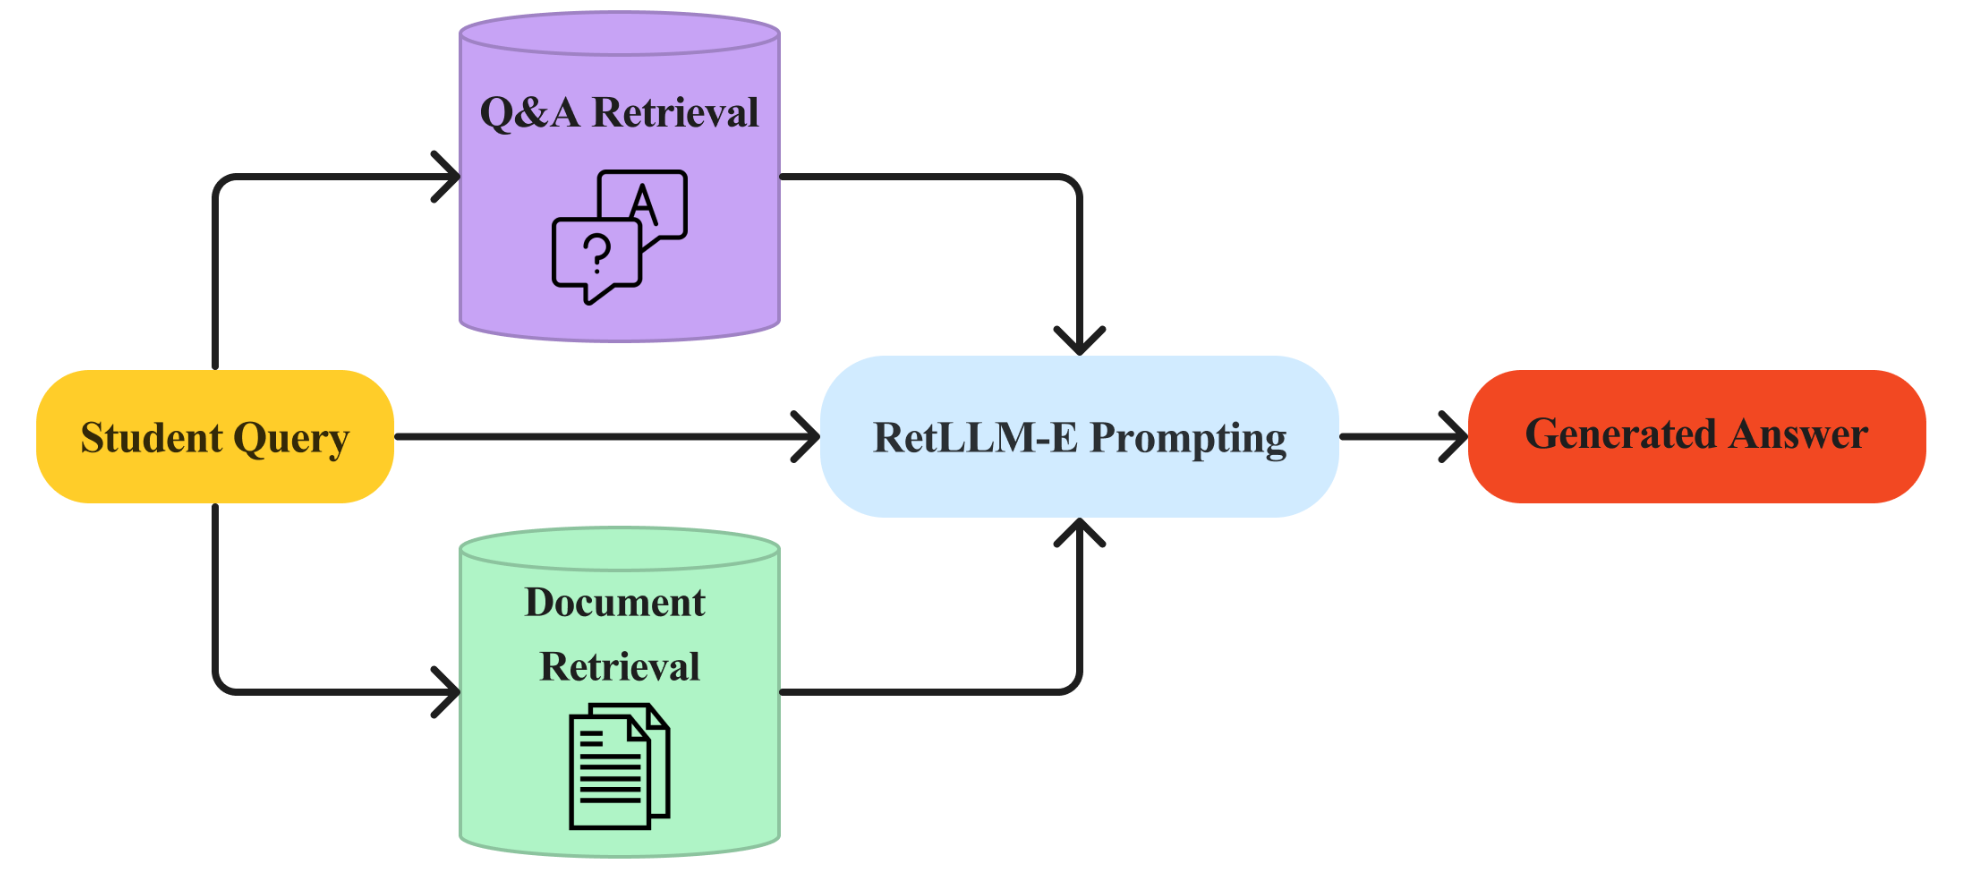
\includegraphics[width=\textwidth]{/root/xzp/Note2024/PaperReading/202406/AAAI/RetLLM-E: Retrieval-Prompt Strategy for Question-Answering on Student Discussion Forums/Images/Figue1.png}
    \caption{Full Pipeline. This figure shows the 3 main parts RetLLM-E \(blue\). The \(i\) question \(yellow\) \(ii\) the document retrieval module \(green\), and \(iii\) the Q\&A retrieval module \(purple\) are incorporated into a prompt-engineered format for the LLM to generate a response \(red\).}
\end{figure}

\subsection{Prompt Details}
\begin{itemize}
    \item Thus, the first part of our prompting strategy is to have the LLM adopt the identity of an appropriate expert, which in this case is a teaching staff in DATA 100.
    \item also precondition the LLM to give answers relevant to the general topics of the class.
    \item precondition the LLM to respond in a “clear, helpful, and positive tone.”
\end{itemize}

In addition to pre-conditing the LLM to take on the identity and style of experienced teaching staff, they tell the LLM not to respond if it is unsure of the answer.

\begin{figure}[H]
    \centering
    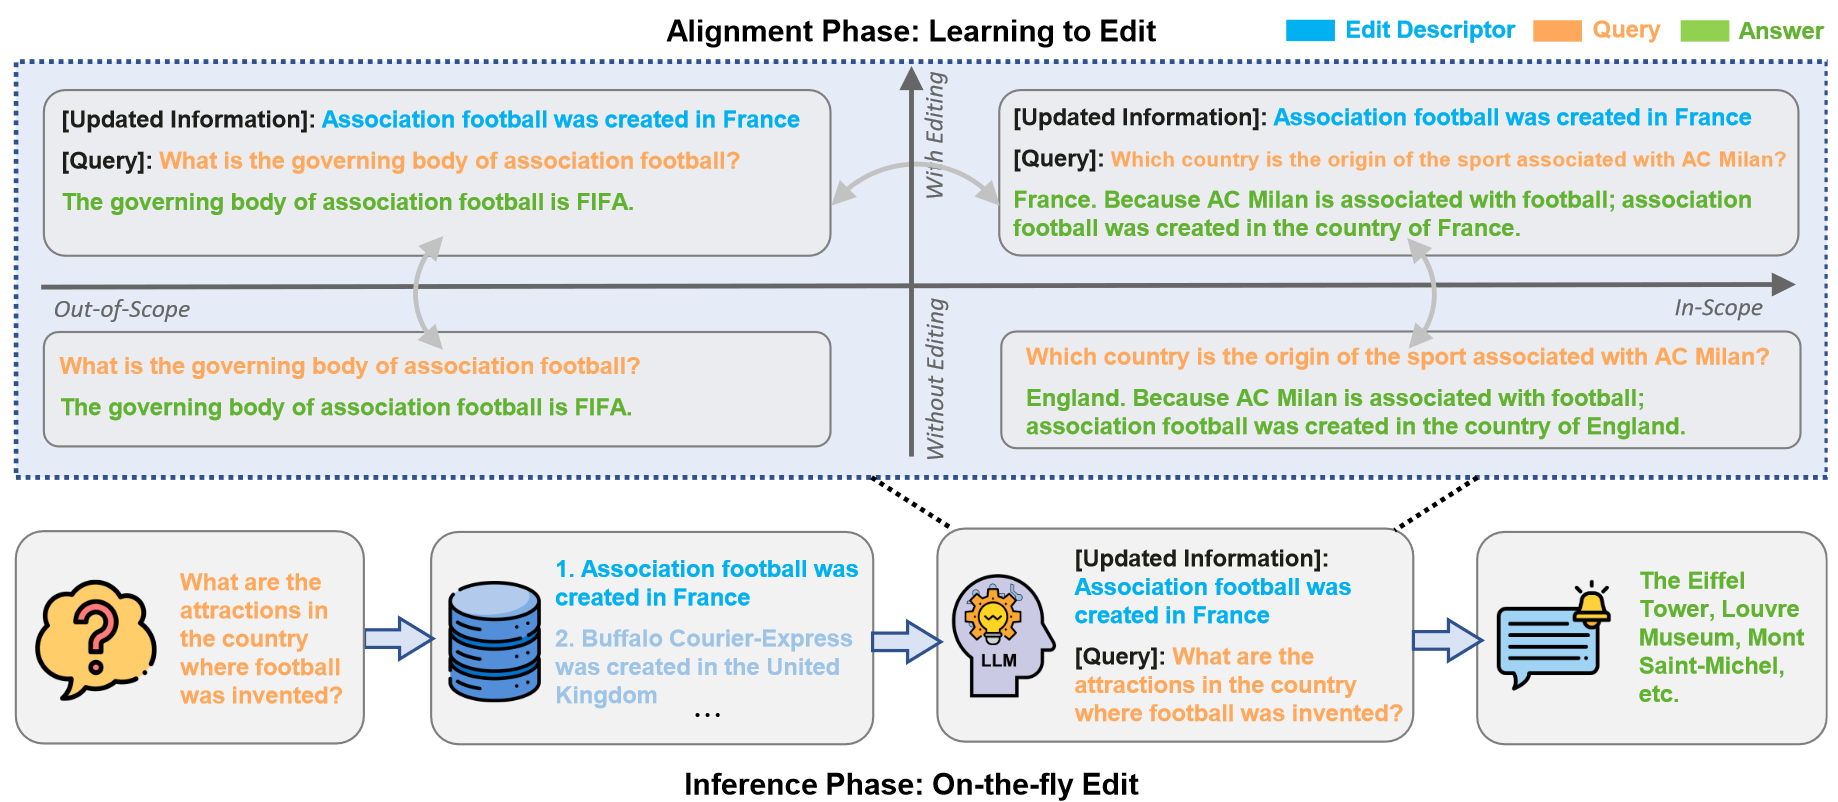
\includegraphics[width=\textwidth]{/root/xzp/Note2024/PaperReading/202406/AAAI/RetLLM-E: Retrieval-Prompt Strategy for Question-Answering on Student Discussion Forums/Images/Figure2.png}
    \caption{RetLLM-E Prompt. The prompt structure of RetLLM-E is outlined. In addition to the key elements of Q\&A context, document context, and the student question, we include prompt-engineering methods to provide tailored responses to students\textquotesingle{} questions and not reinforce misconceptions if the LLM is unsure of the answer.}
\end{figure}

\section{DataAnalysis, Applications, Conclusion and Future Work}

\textbf{Evaluation:} The authors evaluate their system in the context of the EdSTEM discussion forum for UcB's course DATA 100. The cleaned and processed dataset contains 6016 QA pairs.
They formatted the raw anonymized content to optimize the data for retrieval tasks. Each structured data point, or Q\&A pair, comprises the student question, the corresponding staff response, and key post details from EdSTEM
(the post title and the associated context from prior conversations under the same thread).

\section{Why is it published in AAAI?}


\end{document}